\documentclass[10pt]{article}

\usepackage[top=4.3cm,bottom=4.3cm,left=4.8cm,right=4.8cm]{geometry}
\usepackage{newtxtext,newtxmath}
\usepackage{setspace}
\usepackage{graphicx}
\usepackage{booktabs}
\usepackage{array}
\usepackage{microtype}
\usepackage[numbers,sort&compress]{natbib}
\usepackage[hidelinks]{hyperref}
\usepackage{xurl}
\usepackage{enumitem}

\doublespacing
\setlength{\parindent}{1.5em}
\setlength{\parskip}{0pt}
\setcounter{page}{1}

\title{Drug-Cold Gains Do Not Persist under Scaffold Separation in ncRNA--Drug Prediction}
\author{Jihao Li\\
  \small Independent Researcher, Shenzhen, Guangdong, China\\
  \small Corresponding author: Jihao Li, Shenzhen, Guangdong, China; \href{mailto:jihao.li@polyu.edu.hk}{jihao.li@polyu.edu.hk}}
\date{}

\begin{document}
\maketitle

\begin{abstract}
Drug--non-coding RNA (ncRNA) association models are often evaluated using random pair splits or ordinary entity cold-start protocols. However, holding out drug identities does not establish extrapolation to unseen chemical scaffolds. We froze and compared two protocols: the public RAHGL-MDR ordinary drug-cold full-candidate ranking and a strict split with no Bemis--Murcko scaffold shared across training, validation, and test sets. On the fixed RAHGL-MDR folds, an entity-balanced prior-residual candidate achieved a drug-macro average precision (AP) of 0.184244 versus 0.170664 for a training-only RNA-frequency prior, a gain of 0.013580 (95\% paired-bootstrap interval, 0.005139--0.024170; non-decreasing in 5/5 folds). Under the scaffold-disjoint protocol, candidate and prior AP were 0.175435 and 0.175139, respectively, yielding a gain of 0.000296 (scaffold-cluster 95\% interval, $-0.007782$--0.008476; non-decreasing in 2/5 folds), with one of three training seeds producing a negative gain. On the Mi data, the candidate exceeded strict adaptations of LocalGL, a sequence-free sChemNET ablation, and PLMF-MDA, but improved over the RNA prior by only 0.004239, below the prespecified 0.01 materiality threshold. Cross-database de-overlap also changed the ncRNADrug gain from 0.007581 to $-0.012729$. The supported conclusion is conditional: the candidate improves new-drug ranking under the fixed ordinary drug-cold protocol, but the present scaffold-disjoint evaluation does not confirm robust gain for unseen chemical cores. New-drug studies should jointly report full-candidate ranking, strong frequency priors, scaffold separation, and source-overlap audits.
\end{abstract}

\noindent\textbf{Keywords:} ncRNA--drug association; drug cold start; scaffold-disjoint split; full-candidate ranking; frequency prior; evaluation protocol

\section{Introduction}

Drug--ncRNA association prediction seeks to recover or extend potentially relevant associations from previously reported relations. The task lies between interaction prediction and retrieval: for each drug, a model must rank a large candidate set in which reported positives are sparse and unreported pairs remain unlabeled. Related RNA--small-molecule systems range from feature encoders and affinity regressors to structure-based virtual screening and sequence-based interaction scoring \citep{wang2023rnaincoder,oliver2020rnamigos,carvajalpatino2025rnamigos2,krishnan2024rsapred,ma2025rnasmol}. Their inputs, endpoints, negative constructions, and candidate spaces differ, so a numerical comparison outside a common protocol would be misleading.

Recent ncRNA--drug work has used graph neural networks, local subgraphs, multi-view representations, and biological language models, while evaluation has expanded from random pair splits to drug-cold, RNA-cold, and double-cold protocols. These protocols answer different questions. A random pair split allows training and test sets to share entities. An ordinary drug-cold split withholds test-drug identities but does not require their chemical scaffolds to be absent from training. A scaffold-disjoint split imposes the stronger condition that the structural cores of test drugs are unseen. This distinction parallels long-standing warnings in drug--target prediction that random pair, unseen-drug, unseen-target, and double-unseen settings estimate different deployment problems \citep{pahikkala2015realistic}. Without distinguishing these levels, evidence for ``new-drug prediction'' can be interpreted as the stronger and unsupported claim of extrapolation to new chemical scaffolds.

A second issue is the strength of simple priors. In full-candidate ranking, reporting frequencies differ markedly across RNAs. Ranking candidates only by RNA frequency in the training set can therefore provide a strong drug-independent baseline. A model may outperform more complex public neural systems while adding little over this prior. Likewise, database-level validation may reuse RNAs, drugs, and positive pairs. Calling a second database independent without auditing these overlaps can overstate the evidence.

This study does not propose a universally superior algorithm. Instead, it freezes a conditional question: can an entity-balanced prior-residual ranker reliably improve full-candidate ranking for unseen drug identities under an ordinary drug-cold protocol, and does that advantage persist under strict separation of chemical scaffolds? We additionally use Mi, ncRNADrug, NoncoRNA, a historical SM2miR snapshot, and labels supported by distinct PubMed identifiers to examine how strong priors, structural separation, entity overlap, and source independence affect the conclusion \citep{cao2024ncrnadrug,li2020noncorna,liu2013sm2mir}.

The contributions are:
\begin{enumerate}[leftmargin=*]
  \item a frozen conditional result: a 0.013580 AP gain over the RNA prior on the fixed RAHGL-MDR drug-cold folds versus a 0.000296 gain with an interval crossing zero under the present scaffold-disjoint protocol;
  \item an evaluation ladder separating random-pair, entity-cold, scaffold-cold, temporal-new-drug, and independent-source targets under a common full-candidate drug-macro AP endpoint;
  \item strict common-endpoint adaptations of ncRD-LG LocalGL, a sequence-free sChemNET ablation, and PLMF-MDA, with explicit boundaries between original implementations and independent adaptations;
  \item quantified entity and positive-pair overlap between Mi and ncRNADrug, together with de-overlap, temporal-new-drug, and distinct-PubMed analyses; and
  \item a local evidence package that rebuilds the frozen main table and figures and records failed routes and prohibited claims.
\end{enumerate}

\begin{figure}[htbp]
  \centering
  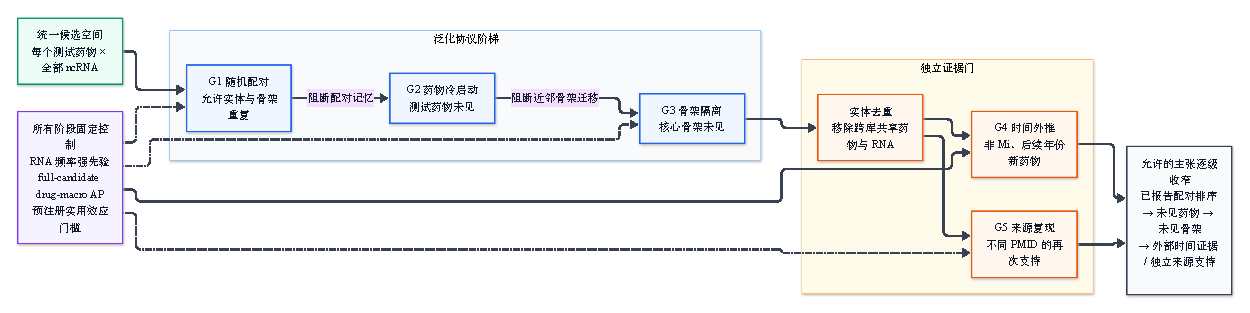
\includegraphics[width=\linewidth]{figures/evaluation-ladder.pdf}
  \caption{Evaluation ladder and evidence boundary. Each higher level changes the estimand rather than merely making the same test more difficult. The present main comparison freezes ordinary drug-cold and strict scaffold-disjoint protocols; temporal and source-independent analyses are boundary checks rather than equivalent replications.}
  \label{fig:ladder}
\end{figure}

\section{Related work}

\subsection{RNA--small-molecule and ncRNA--drug prediction}

RNA--small-molecule prediction spans several non-equivalent tasks. RNAincoder learns compressed representations from hundreds of RNA descriptors and thousands of compound descriptors, then evaluates downstream RNA-associated classification problems \citep{wang2023rnaincoder}. RNAmigos instead predicts ligand fingerprints from three-dimensional RNA-pocket graphs and ranks a native ligand among property-matched decoys \citep{oliver2020rnamigos}. RNAmigos2 scales this structure-based setting with docking supervision and binding-site cluster separation, but its structural-pocket split is not a drug-scaffold split over a full ncRNA candidate space \citep{carvajalpatino2025rnamigos2}. RSAPred treats experimentally collected RNA--small-molecule affinities as a regression problem and evaluates cross-validation, jackknife, and external sets \citep{krishnan2024rsapred}. RNAsmol is a sequence-based classifier that explicitly reports RNA-cold, small-molecule-cold, double-cold, and decoy-ranking evaluations \citep{ma2025rnasmol}. These studies establish valuable RNA--ligand modeling precedents, but they do not make their metrics interchangeable with full-candidate drug-macro AP on association databases.

ncRD-LG combines biological language models with local semantic subgraphs for drug--ncRNA association prediction. Its principal protocol is a random pair-level split, while leave-one-drug-out, leave-one-ncRNA-out, and scaffold-based splitting are identified as future evaluation directions \citep{xie2026ncrdlg}. RAHGL-MDR evaluates leakage-controlled edge, miRNA-cold, drug-cold, and double-cold settings and includes full-candidate ranking and degree/popularity baselines \citep{elbashir2026rahgl}. Cold-start evaluation and full-candidate ranking are therefore not new in this study.

HMVCC reports edge-level, cross-species, cross-database, and drug-cold settings for ncRNA--drug association prediction \citep{ma2027hmvcc}. MGCNA learns multi-view graph-convolutional representations for miRNA--drug association prediction \citep{sheng2025mgcna}. PLMF-MDA combines RNA-FM, ChemBERTa-2, intrinsic encoders, and cross-modal attention for miRNA--drug resistance and sensitivity associations \citep{sheng2026plmf}. sChemNET directly studies small molecules targeting microRNA function and evaluates chemically dissimilar test subsets using a molecular-fingerprint similarity threshold; its reported protocol is not a Bemis--Murcko scaffold split \citep{galeano2024schemnet}. The public GCFMCL implementation uses drug-as-user Bayesian personalized ranking during representation learning; we therefore do not claim to introduce pairwise ranking for this task \citep{wei2023gcfmcl}.

\subsection{Pretrained representations and cold-start transfer}

Large pretrained encoders can supply information that is absent from a sparse association matrix. RNA-FM uses self-supervised learning over 23 million non-coding RNA sequences and evaluates structure and function tasks \citep{chen2022rnafm}; RNAErnie adds motif-aware pretraining and type-guided fine-tuning \citep{wang2024rnaernie}; and BiRNA-BERT studies nucleotide- and BPE-level tokenization across several RNA tasks \citep{tahmid2025birnabert}. On the chemical side, ChemBERTa pretrains a Transformer on large SMILES corpora and evaluates molecular-property benchmarks, including scaffold-split tasks \citep{chithrananda2020chemberta}. These works motivate transferable features, but representation pretraining alone does not establish scaffold-level generalization for ncRNA--drug association ranking.

The drug--target literature makes the same boundary visible. GraphDTA combines molecular graphs with protein-sequence encoders but uses standard pair splits on Davis and KIBA \citep{nguyen2021graphdta}. TransDTI evaluates language-model representations for drug--target interaction classification and regression \citep{kalakoti2022transdti}. C2P2 explicitly separates cold-drug and cold-target entities and transfers auxiliary chemical--chemical and protein--protein interaction knowledge \citep{nguyen2022coldstartdta}. DrugBAN reports random, unseen-entity, cold-pair, and clustering-based cross-domain splits; importantly, it observes that an identity-level unseen-drug split can remain easy when close chemical analogues cross the partition \citep{bai2023drugban}. Thus, entity novelty and chemical-core novelty require separate controls.

\subsection{Local subgraphs, ranking objectives, and evaluation design}

Learning from an enclosing subgraph is a general link-prediction strategy rather than an ncRNA--drug-specific invention. SEAL formalizes how local enclosing subgraphs can approximate broad classes of link heuristics and jointly uses structure, embeddings, and attributes \citep{zhang2018seal}. Likewise, Bayesian personalized ranking was introduced for pairwise optimization from implicit feedback, where missing entries are not assumed to be verified negatives \citep{rendle2009bpr}. Our local-subgraph comparators and pairwise residual objective should be understood as task-specific adaptations of these precedents.

Evaluation design is equally consequential. Pahikkala et al. separate pair-wise, unseen-drug, unseen-target, and double-unseen settings and show why splitting at the wrong level can give optimistic estimates \citep{pahikkala2015realistic}. MoleculeNet similarly warns that random splitting is often inappropriate for chemical data and defines scaffold grouping as a stronger structural-separation test \citep{wu2018moleculenet}. For imbalanced retrieval, precision--recall analysis exposes false-positive burden that can be visually obscured in ROC space, and optimizing ROC area does not guarantee optimizing PR area \citep{davis2006prroc,saito2015pr}. These observations motivate our full-candidate drug-macro AP endpoint and the separation of identity-cold from scaffold-disjoint claims.

\subsection{Identifier and evidence provenance}

Association benchmarks inherit the scope and uncertainty of their source databases. miRBase provides stable microRNA nomenclature but also documents variable annotation confidence \citep{kozomara2014mirbase}; Rfam represents RNA families through curated alignments, consensus structures, and covariance models rather than drug-response labels \citep{kalvari2021rfam}. PubChem aggregates depositor-supplied chemical records and standardizes structures while preserving distinctions between Substance and Compound records \citep{kim2023pubchem}. RNAInter integrates experimental and computational interactions and assigns evidence-derived confidence scores, so an entry's presence and score do not turn every absent pair into a verified negative \citep{kang2022rnainter}. lncRNAdb emphasizes manually curated functional evidence for a comparatively small set of characterized lncRNAs \citep{quek2015lncrnadb}, whereas DrugBank combines curated and predicted drug information under source- and use-specific access terms \citep{wishart2018drugbank}. These differences justify explicit normalization, provenance fields, and overlap audits rather than treating database names as interchangeable evidence.

As of the freeze date, our bounded full-text review found no single direct neighbor that jointly reports Bemis--Murcko scaffold separation, full-candidate drug-macro AP, a training-only RNA-frequency prior, cross-database entity de-overlap, temporal-new-drug evidence, and labels supported by distinct PubMed identifiers in one ncRNA--drug audit. This is a provisional gap under a bounded search, not a claim of priority or exhaustive absence.

\section{Methods}

\subsection{Task and estimand}

Given reported positive ncRNA--drug associations in a training set, the model scores the full set of candidate ncRNAs for each held-out drug. The primary metric is average precision for each drug, macro-averaged over test drugs. Database-unrecorded pairs are treated as unlabeled candidates, not as experimentally verified biological negatives.

We distinguish two main protocols. In \textbf{ordinary drug-cold} evaluation, drug identities are mutually exclusive across training, validation, and test sets, but scaffolds are not forced to be disjoint. We interpret this only as entity cold start on the fixed RAHGL-MDR folds. In \textbf{strict scaffold-disjoint} evaluation, Bemis--Murcko scaffolds define groups that do not overlap across training, validation, and test sets; acyclic molecules are grouped by canonical SMILES. This protocol represents a stronger unseen-core requirement.

Ordinary drug-cold evaluation does not imply that every test drug shares a training scaffold, and it is not equivalent to strict scaffold extrapolation. We compare two frozen protocols and do not attribute their difference to a single leakage mechanism.

\subsection{Protocol hierarchy and split construction}

Table~\ref{tab:protocols} states the claim supported by each split. The hierarchy is not a monotone difficulty scale: changing the split changes which population is tested and can also alter training-set size, class support, and chemical diversity. In particular, identity-disjoint drugs may still share close analogues or the same two-dimensional core with training drugs. We therefore use ``ordinary drug-cold'' only for identity separation and reserve ``scaffold-disjoint'' for the stronger structural condition.

\begin{table}[htbp]
\centering
\caption{Protocol definitions and permitted interpretation. ``Shared'' means that the protocol does not prohibit overlap.}
\label{tab:protocols}
\small
\begin{tabular}{p{0.24\linewidth}p{0.20\linewidth}p{0.20\linewidth}p{0.29\linewidth}}
\toprule
Protocol & Drug identity & Drug scaffold & Supported interpretation \\
\midrule
Random pair & Shared & Shared & Missing pairs among previously represented entities \\
Drug-cold & Disjoint & May be shared & Ranking for unseen drug identities in the sampled chemical space \\
Double-cold & Disjoint & May be shared & Pairs whose drug and RNA identities are both unseen \\
Scaffold-disjoint & Disjoint & Disjoint & Ranking for held-out two-dimensional chemical cores under the constructed split \\
Temporal new-drug & Time-ordered & Unconstrained & Performance on drugs appearing after the training cutoff \\
\bottomrule
\end{tabular}
\end{table}

The ordinary drug-cold folds are the fixed public RAHGL-MDR folds. The strict protocol computes one Bemis--Murcko framework per standardized molecule and assigns whole framework groups to a single outer partition. This follows the chemical-learning rationale that a scaffold split separates structurally different molecules more strongly than a random split \citep{wu2018moleculenet}. Acyclic molecules lack a conventional ring framework, so we group them by canonical SMILES instead of collapsing all such compounds into one artificial scaffold. All group labels are computed before model fitting, and validation data are used only for the frozen candidate choices described below.

\subsection{Data and candidate spaces}

The RAHGL-MDR data contain 635 miRNAs, 216 drugs, and 5,379 unique positive pairs; 197 drugs with at least one positive association enter the drug-cold or scaffold-cold outer tests. The aligned Mi artifact contains 1,805 ncRNAs, 625 drugs, and 9,395 positive pairs, with 606 active drugs entering the principal scaffold-disjoint evaluation. ncRNADrug, NoncoRNA, a temporal subset from SM2miR, and a Mi subset supported by distinct PubMed identifiers are used for boundary analyses. Detailed counts and provenance-field availability are supplied in the supplementary dataset/protocol table.

All primary evaluations enumerate every ncRNA candidate for each test drug. Overlap between Mi and ncRNADrug is computed using frozen normalization rules for RNA names, drug names, and positive pairs. The de-overlap confirmation removes entities that match Mi; it does not selectively remove pairs after observing model scores.

RNA identifiers are normalized against the identifiers and aliases available in the frozen artifacts; miRNA and RNA-family terminology is checked against the roles documented by miRBase and Rfam \citep{kozomara2014mirbase,kalvari2021rfam}. Drug strings and available compound identifiers are standardized before overlap comparison, with PubChem serving as the reference model for distinguishing depositor records from standardized compound structures \citep{kim2023pubchem}. Database provenance is retained because RNAInter mixes evidence types, lncRNAdb is manually curated around functional literature, and DrugBank contains both curated and predicted fields \citep{kang2022rnainter,quek2015lncrnadb,wishart2018drugbank}. Identifier normalization reduces superficial mismatches; it does not harmonize biological assays or make missing associations negative.

\subsection{Candidate and strong baseline}

The RNA prior is estimated only from RNA positive counts among inner-training drugs and uses Laplace smoothing. The candidate learns a pairwise residual over this prior from drug and RNA features. For the RAHGL-MDR main analysis, each training drug contributes equally to total pairwise loss, preventing drugs with more observed edges from dominating the objective. A residual scale is selected from a frozen grid using only the inner validation set; a scale of zero exactly recovers the RNA prior.

We do not claim that this objective is a novel ranking loss. GCFMCL already uses Bayesian personalized ranking during representation learning. Here the candidate tests whether entity-balanced training improves a specific drug-cold distribution rather than establishing universal algorithmic novelty.

The pairwise residual is trained from observed-versus-unobserved candidate orderings. This use of an implicit-feedback ranking objective follows the basic distinction in BPR between observed positives and unobserved entries \citep{rendle2009bpr}; it does not assert that sampled unobserved pairs are experimentally confirmed negatives. The model's drug-specific component can therefore be interpreted only as a ranking correction to the training-only RNA prior.

\subsection{Comparators and implementation boundaries}

The strict Mi endpoint includes a dynamically resampled adaptation of ncRD-LG LocalGL, an sChemNET ablation without miRNA sequence information or external unlabeled-drug augmentation, and an independent three-seed strict adaptation of PLMF-MDA. The sChemNET and PLMF-MDA results are not reproductions of the original reported numbers. RAHGL-MDR does not release its training implementation and per-candidate predictions; we therefore reuse its public data and fixed folds for diagnostic baselines but do not make a paired head-to-head claim against the authors' trained model.

\subsection{Statistical analysis and freeze rules}

Average precision is computed separately for each held-out drug across its complete ncRNA candidate list and then macro-averaged, giving each evaluated drug equal weight. PR-based summaries are appropriate here because reported associations are rare relative to the enumerated candidate space and false positives directly reduce precision \citep{davis2006prroc,saito2015pr}. AUROC is not used as the primary endpoint, and AP values from restricted or balanced negative sets are not treated as comparable to full-candidate AP.

For ordinary RAHGL-MDR drug-cold evaluation, paired bootstrap resampling operates over drug-level differences. For strict scaffold-cold evaluation, bootstrap resampling is clustered by scaffold group. Both main RAHGL-MDR protocols report 95\% intervals, the number of non-decreasing folds, and three training seeds. The frozen strict-scaffold confirmation gate requires an AP gain of at least 0.01 over the RNA prior, a confidence-interval lower bound above zero, non-decrease in at least four of five folds, positive gains for all three seeds, and gains of at least 0.01 for at least two seeds. An earlier ordinary drug-cold gate additionally required exceeding the popularity MAP reported in RAHGL-MDR.

The intervals are conditional on the fixed outer partition and the executed training seeds. Seed-specific AP is first averaged for the same fold and drug; drugs or scaffold groups are then resampled. The intervals do not integrate uncertainty from drawing new training seeds or new outer partitions. Auxiliary analyses use their own frozen configurations and decision gates.

All new exploration, training, data download, and hyperparameter tuning stopped on 20 October 2026. Post-freeze work is limited to rebuilding existing tables and figures, verifying hashes and tests, checking citations, and preparing submission material. Bootstrap intervals do not remove historical method-selection bias; Mi results are therefore labelled developmental evidence.

\section{Results}

\subsection{Ordinary drug-cold gain did not persist under the strict scaffold evaluation}

Across three training seeds on the fixed RAHGL-MDR drug-cold folds, the entity-balanced prior-residual candidate achieved an AP of 0.184244 versus 0.170664 for the RNA prior. The difference was 0.013580, with a 95\% interval of 0.005139--0.024170 and non-decrease in all five folds. The candidate passed the frozen ordinary drug-cold gate.

With the same data source, candidate space, model family, and training seeds but a newly constructed five-fold scaffold-disjoint protocol, candidate AP was 0.175435 and prior AP was 0.175139. The gain fell to 0.000296, with a scaffold-cluster 95\% interval of $-0.007782$--0.008476 and non-decrease in only two of five folds. Seed-specific gains were 0.005339, 0.008217, and $-0.012667$. Relative to the same-budget ordinary pairwise variant, the entity-balanced candidate gained only 0.000857 and the interval crossed zero.

The two protocols also change the composition of training, validation, and test drugs. These observations do not identify scaffold separation as the sole causal mechanism. They support the narrower conclusion that the positive result under the fixed ordinary drug-cold protocol was not robustly confirmed in the present strict scaffold-disjoint evaluation.

\begin{figure}[htbp]
  \centering
  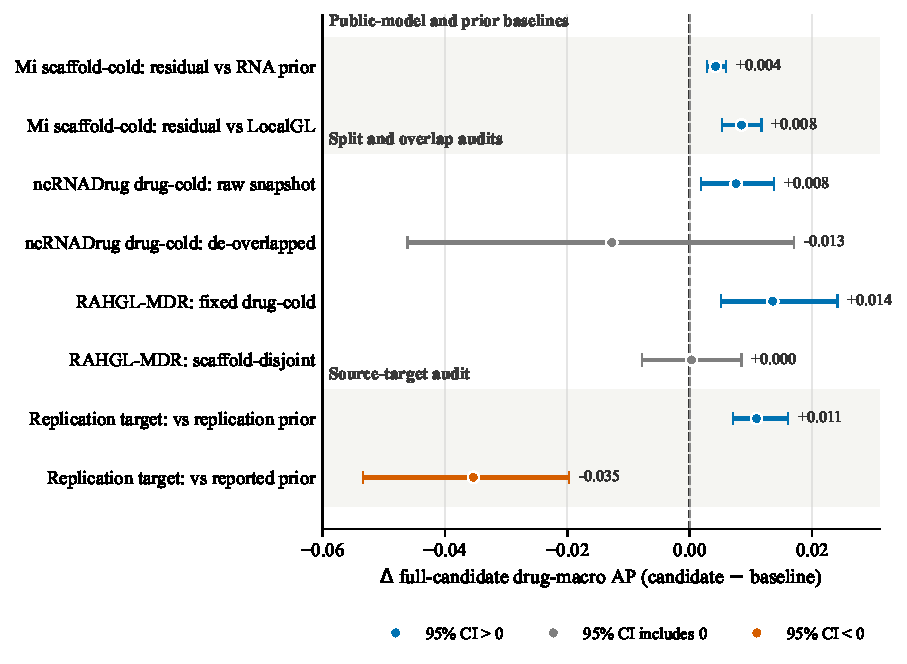
\includegraphics[width=\linewidth]{figures/fig_conclusion_reversals.pdf}
  \caption{Protocol- and source-dependent changes in the candidate-minus-prior AP difference. Intervals are conditional on the frozen splits and executed seeds. The figure does not estimate a universal treatment effect of scaffold separation.}
  \label{fig:reversals}
\end{figure}

\begin{table}[htbp]
\centering
\caption{Frozen primary comparisons. AP is drug-macro average precision over the full candidate set.}
\label{tab:main}
\small
\begin{tabular}{p{0.47\linewidth}rrr}
\toprule
Comparison & Candidate & Baseline & Difference \\
\midrule
RAHGL ordinary drug-cold vs RNA prior & 0.184244 & 0.170664 & 0.013580 \\
RAHGL scaffold-disjoint vs RNA prior & 0.175435 & 0.175139 & 0.000296 \\
Mi scaffold-disjoint vs RNA prior & 0.161748 & 0.157509 & 0.004239 \\
Mi second scaffold split vs RNA prior & -- & -- & 0.002881 \\
Mi vs dynamic LocalGL & 0.161748 & 0.153275 & 0.008473 \\
Mi vs sChemNET no-sequence ablation & 0.161748 & 0.154500 & 0.007248 \\
Mi vs independent PLMF-MDA adaptation & 0.161748 & 0.135050 & 0.026698 \\
ncRNADrug original vs RNA prior & 0.114019 & 0.106438 & 0.007581 \\
ncRNADrug de-overlapped vs RNA prior & 0.063689 & 0.076418 & $-0.012729$ \\
NoncoRNA vs RNA prior & 0.109175 & 0.105596 & 0.003579 \\
SM2miR temporal mini-holdout vs prior & -- & -- & $-0.019876$ \\
\bottomrule
\end{tabular}
\end{table}

\subsection{Beating public neural adaptations did not imply a material gain over the strong prior}

On the main five-fold Mi scaffold-disjoint evaluation, candidate AP was 0.161748 and RNA-prior AP was 0.157509. The gain was 0.004239 (95\% interval, 0.002812--0.005899), with non-decrease in all five folds, but it did not reach the 0.01 materiality gate. A second scaffold split produced a gain of 0.002881 (95\% interval, 0.001047--0.004782) and non-decrease in four of five folds, also failing the gate.

On the same candidate space and scaffold endpoint, AP values for dynamic LocalGL, the sequence-free sChemNET ablation, and the independent strict PLMF-MDA adaptation were 0.153275, 0.154500, and 0.135050. The candidate was higher by 0.008473, 0.007248, and 0.026698, respectively. Each public-method summary used its matched prior, approximately 0.157507; this differs from the main-table prior of 0.157509 by about $1.8\times10^{-6}$ and does not change the conclusion. The candidate's practically relevant increment over the strong prior remained below 0.01. Thus, outperforming complex neural adaptations and adding material drug-specific information over a frequency prior are distinct claims.

\subsection{Cross-database overlap changed the external-validation conclusion}

The aligned Mi and ncRNADrug snapshots share RNAs, drugs, and positive pairs. Under the original ncRNADrug drug-cold evaluation, the candidate gained 0.007581 over the prior (95\% interval, 0.001838--0.013747) and was non-decreasing in all five folds. After removing entities matched to Mi, candidate AP was 0.063689 and prior AP was 0.076418, producing a gain of $-0.012729$ with an interval crossing zero. The confirmation gate failed. On NoncoRNA, the gain was 0.003579, its interval also crossed zero, and only two of five folds were non-decreasing.

De-overlap does not prove that the original positive result was caused entirely by leakage because it also changes sample composition and support. It does show that a second database with unaudited entity and pair overlap cannot automatically be treated as independent confirmation.

\subsection{Temporal drugs and source-derived labels exposed additional boundaries}

On a temporal mini-holdout of 18 SM2miR compounds whose CIDs did not occur in Mi, the candidate underperformed the prior by 0.019876. The small subset rules out positive confirmation for this test but cannot estimate a universal external effect.

For Mi pairs supported by at least two distinct PubMed identifiers, an ECFP residual trained directly on the replicated-literature label gained 0.010933 over the frequency prior estimated for that label, but underperformed the RNA prior estimated from all reported pairs by 0.035344. The interaction-hurdle model selected zero weight in all five folds and therefore exactly recovered its first stage; the conditional-prior hurdle selected non-zero weight only in fold 2. Distinct PubMed identifiers are not equivalent to independent experimental replication and do not identify a causal reporting mechanism.

\section{Discussion}

\subsection{Conditional contribution}

The strongest supported claim is deliberately narrow. Under the fixed RAHGL-MDR ordinary drug-cold partition, the candidate reliably improves full-candidate ranking. The present strict scaffold-disjoint evaluation does not confirm a comparably robust advantage. The ordinary drug-cold result is evidence for the evaluated entity-cold protocol. It is insufficient for a claim about unseen chemical cores.

\subsection{Why the strong prior must be retained}

The RNA-frequency prior reflects reporting structure rather than a biological mechanism. Precisely because association databases are highly imbalanced, it is a necessary control for whether a model adds drug-specific information. On Mi, the candidate significantly exceeded several neural adaptations yet improved AP over the prior by less than 0.005. Comparisons only among complex methods can therefore obscure the practically central baseline.

\subsection{Mechanisms not identified by the results}

The difference between ordinary drug-cold and scaffold-disjoint results cannot be attributed simply to same-scaffold leakage. Repartitioning by scaffold changes structural support, training composition, and the outer test distribution simultaneously. The study was not designed to identify separate causal effects for those factors and does not select models after inspecting post hoc strata.

\subsection{Reporting recommendations}

Studies that target new-drug ncRNA--drug prediction should report full-candidate drug-macro AP; a frequency prior estimated from training data only; both ordinary drug-cold and scaffold-disjoint results; train--test overlap in entities, scaffolds, and positive pairs; multiple split and training seeds; uncertainty clustered by drug or scaffold; a clear separation between original-model reproduction and independent adaptation; and the fact that unknown pairs are unlabeled.

\subsection{Limitations}

First, multiple candidates were developed on Mi, and the reported intervals do not remove historical method-selection bias. Second, RAHGL-MDR does not release its training code and per-candidate predictions, preventing a paired same-implementation reproduction of the authors' model. Third, the ordinary drug-cold and scaffold-disjoint protocols use different outer assignments and therefore represent performance under different conditions rather than a single-drug counterfactual. Fourth, ncRNADrug triples lack pair-level PubMed identifiers, limiting source-independence checks. Fifth, the temporal SM2miR subset is small. Sixth, all labels are drawn from reported associations; no prospective or wet-laboratory validation was conducted. Seventh, several upstream repositories lack an explicit license. The evidence package is therefore not a complete training-data release.

\section{Conclusion}

On the fixed RAHGL-MDR ordinary drug-cold folds, an entity-balanced prior-residual candidate produced a stable gain above the frozen materiality threshold for full-candidate ncRNA ranking. Under the present strict scaffold-disjoint split, the gain was near zero, its interval crossed zero, and its sign was unstable across seeds. Together with strong-prior comparisons on Mi, cross-database de-overlap, and source-derived-label audits, the evidence supports one conditional claim: \textbf{a gain exists under the fixed ordinary drug-cold protocol, but that performance claim cannot be directly extended to unseen chemical scaffolds.} This boundary is more faithful to the current evidence than a universal algorithmic claim and provides concrete requirements for future evaluation.

\section*{Data and code availability}

The public evidence package contains frozen summaries/configurations, the main table and figures, rebuilding scripts, tests, a third-party boundary, and a SHA-256 manifest. Third-party raw data, repository code, model weights, and paper PDFs are not redistributed. Repository: \url{https://github.com/ljhOfGithub/ncrna-drug-generalization-audit}; versioned release: \url{https://github.com/ljhOfGithub/ncrna-drug-generalization-audit/releases/tag/v0.1.3}. A permanent archive DOI has not yet been assigned.

\section*{Ethics statement}

This computational study used public or lawfully accessed data and involved no new participant recruitment, intervention, animal experiment, or identifiable individual-level information. Ethical approval and informed consent were therefore not applicable.

\section*{CRediT authorship contribution statement}

Jihao Li: Conceptualization, Methodology, Software, Validation, Formal analysis, Investigation, Data curation, Writing--original draft, Writing--review and editing, Visualization, and Project administration.

\section*{Declaration of competing interest}

The author declares no competing interests.

\section*{Funding}

This research received no specific grant from any funding agency in the public, commercial, or not-for-profit sectors.

\section*{Declaration of generative AI and AI-assisted technologies}

During manuscript preparation, the author used OpenAI Codex to assist literature discovery, code drafting and inspection, execution support, statistical-result checking, manuscript drafting, language editing, citation checking, and consistency checks. The author reviewed and edited all outputs, verified citations and reported numerical results against source materials and saved machine-readable results, and takes full responsibility for the content of the publication. Generative AI was not listed as an author and was not used to create or alter primary research data.

\bibliographystyle{unsrtnat}
\bibliography{references}

\appendix
\section{Submission boundary}

The English manuscript is derived from a frozen Chinese factual source. No post-freeze experiment, retraining, download, or hyperparameter search contributes to the reported results. The public package excludes all upstream raw data, repository clones, model weights, caches, and publisher files. Release \texttt{v0.1.3} is the frozen evidence-package version; a future archival deposit must preserve this version and its manifest.

\section{Interpretation guardrails}

The following statements are not supported by the evidence: universal superiority over ncRNA--drug predictors; state-of-the-art performance under incompatible protocols; proof that scaffold leakage is the sole explanation for the observed difference; a prospective biological validation; or a claim that unknown database pairs are true negatives. The sChemNET comparison is an independent no-sequence ablation, not a reproduction of the full author model. The PLMF-MDA comparison is an independent strict adaptation. HMVCC comparisons use released artifacts under a local protocol and do not reproduce the authors' training run.

\end{document}
